\documentclass[journal, a4paper]{IEEEtran}
\usepackage{graphicx,url,amsmath, verbatim, float, moresize}   
\usepackage[brazil]{babel}
\usepackage[utf8]{inputenc}
\usepackage[T1]{fontenc}
\usepackage[compatibility,siunitx,  americanvoltages, americancurrents, americanresistors, europeaninductors, americanports,straightlabels, fetbodydiode, straightvoltages]{circuitikz}
\usepackage{tikz,amsmath, amssymb,bm,color,pgfkeys,siunitx,ifthen,ulem}
\usepackage{pgfplots}
\newcommand\tab[1][1cm]{\hspace*{#1}}
\pgfplotsset{compat=1.14}
\usetikzlibrary{shapes,arrows}
\usetikzlibrary{circuits.ee.IEC}
\usetikzlibrary{arrows}
\usetikzlibrary{backgrounds,calc,positioning}
\ctikzset{tripoles/mos style/arrows}
\ctikzset{
	/tikz/circuitikz/quadpoles/coupler/width=1,%1.3
	/tikz/circuitikz/quadpoles/coupler/height=0.952,%1.3
	/tikz/circuitikz/quadpoles/coupler2/width=1,%1.3
	/tikz/circuitikz/quadpoles/coupler2/height=0.952,%1.3
	/tikz/circuitikz/quadpoles/transformer/width=1.425,%1.5
	/tikz/circuitikz/quadpoles/transformer/height=1.425,%1.5
	/tikz/circuitikz/quadpoles/transformer core/width=1.425,%1.5
	/tikz/circuitikz/quadpoles/transformer core/height=1.425,%1.5
	/tikz/circuitikz/quadpoles/gyrator/width=1.425,%1.5
	/tikz/circuitikz/quadpoles/gyrator/height=1.425,%1.5
	/tikz/circuitikz/monopoles/tlinestub/width=0.1875,%0.25 no effect!
	/tikz/circuitikz/tripoles/american and port/height=0.95,%.8
	/tikz/circuitikz/tripoles/american nand port/height=0.95,%.8
	/tikz/circuitikz/tripoles/american or port/height=0.95,%.8
	/tikz/circuitikz/tripoles/american nor port/height=0.95,%.8
	/tikz/circuitikz/tripoles/american xor port/height=0.95,%.8
	/tikz/circuitikz/tripoles/american xnor port/height=0.95,%.8
	/tikz/circuitikz/bipoles/tline/height=0.4,%0.3
%	/tikz/circuitikz/bipoles/tline/width=1.2,%0.8
	/tikz/circuitikz/bipoles/diode/height=0.375,%
	/tikz/circuitikz/bipoles/diode/width=0.375,%
	/tikz/circuitikz/bipoles/varcap/height=0.375,%
	/tikz/circuitikz/bipoles/varcap/width=0.375,%
	/tikz/circuitikz/tripoles/triac/height=1.05,%
	/tikz/circuitikz/tripoles/triac/width=0.952,%
	/tikz/circuitikz/tripoles/thyristor/height=1.05,%
	/tikz/circuitikz/tripoles/thyristor/width=0.952,%
	/tikz/circuitikz/tripoles/op amp/height=0.952,%
	/tikz/circuitikz/tripoles/op amp/width=1.2,%
	/tikz/circuitikz/tripoles/op amp/font=\footnotesize,
	/tikz/circuitikz/tripoles/gm amp/height=0.952,% 1.7
	/tikz/circuitikz/tripoles/gm amp/width=1.2,% 1.4
	%	/tikz/circuitikz/tripoles/gm amp/font=\footnotesize,
	/tikz/circuitikz/tripoles/plain amp/height=0.952,% 1.7
	/tikz/circuitikz/tripoles/plain amp/width=1.2,% 1.4
	/tikz/circuitikz/bipoles/resistor/voltage/straight label distance/.initial=.8,
	/tikz/circuitikz/bipoles/generic/voltage/straight label distance/.initial=.8,
	/tikz/circuitikz/bipoles/inductor/voltage/straight label distance/.initial=.8,
	/tikz/circuitikz/bipoles/fullgeneric/voltage/straight label distance/.initial=.8,
	/tikz/circuitikz/bipoles/capacitor/voltage/straight label distance/.initial=1.0,
	/tikz/circuitikz/bipoles/thickness=1.6,
}
\ctikzset{v/.append style={/tikz/european voltages}}

\definecolor{netlabelcolor}{rgb}{0, 0, 0.25}
\definecolor{lttotitextcolor}{rgb}{0, 0.0, 0.25}
\definecolor{lttotidrawcolor}{rgb}{0.6, 0.0, 0.6}
\definecolor{netcolor}{rgb}{0, 0, 0}

\pgfkeys{/lt2ti/netlabel/font/.initial= \small}
\pgfkeys{/lt2ti/text/font/.initial= \small}

\pgfkeys{/lt2ti/Net/.style= {netcolor}}
\tikzstyle{dashdotdotted}=[dash pattern=on 3pt off 2pt on \the\pgflinewidth off 2pt on \the\pgflinewidth off 2pt]

\pgfkeys{/lt2ti/VArrow/.style= {->,>=latex}}
\pgfkeys{/lt2ti/SArrow/.style= {->,>=angle 90}}


\begin{document}


	\title{Relatório 1 - Polarização do circuito Cascode}
	\author{Arthur Pimentel, Matheus Farias e Matheus Henrique de Araujo.

    }
	\maketitle

\section{Introdução}

    \tab Como proposto anteriormente, existem diversos tipos de configuração de amplificadores transistorizados. Desta vez, observa-se-á a configuração Cascode. Como exposto em sala, esta configuração é capaz, teoricamente, de oferecer uma banda de passagem maior, o que aproxima este sistema a um filtro passa-altas, resultado desejado para um amplificador ideal com capacitores de acoplamento. Ainda, espera-se obter uma alta impedância de entrada e uma alta impedância de saída. Para esta relação, algumas aproximações foram necessárias e, por isso, necessita-se de uma avaliação experimental para verificar se o modelo representado está de acordo com a realidade. Note-se, ainda, que outras distorções de resultado também são esperadas e impactarão o percentual de verossimilhança do modelo. Estas distorções existem, entre outros motivos, por conta da diferença entre os valores teóricos e práticos dos componentes. %s adaptações dos componentes aos que existem disponível no mercado. Por exemplo, os resistores não são aqueles usados no projeto, mas sim os de valores nominais mais próximos encontrados pelo grupo.

\section{Análise Teórica}
	\subsubsection{Projeto}
	
	    \tab No design do amplificador desejado, inicialmente, foi fornecido o modo de polarização do circuito Cascode. Observa-se, na Figura %\ref{modelo}, a configuração fornecida para o projeto.
	        
	    \begin{figure}[H]
            \begin{center}
            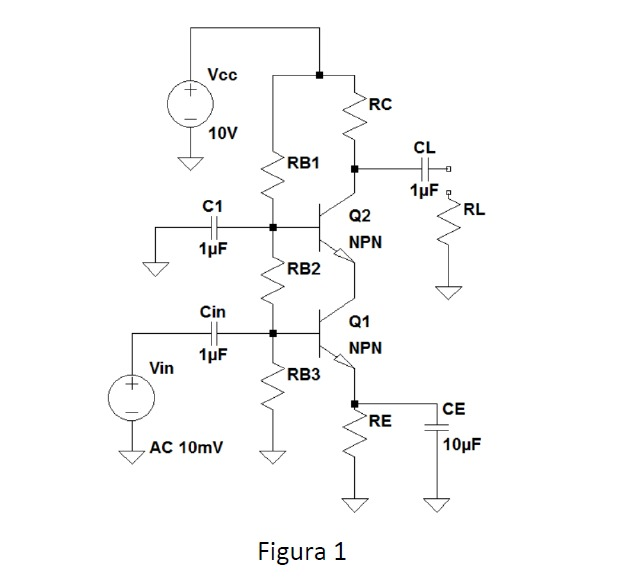
\includegraphics[width=\columnwidth]{Cascode.png}
            \caption{Esquema do circuito Cascode}
            \label{Cascode}
            \end{center}
        \end{figure}  
	        %\makeatletter

%% bandstop filter (adapted from highpass)
\pgfcircdeclarebipole{}{\ctikzvalof{bipoles/highpass/width}}{*bandstop}{\ctikzvalof{bipoles/highpass/width}}{\ctikzvalof{bipoles/highpass/width}}{
	\pgf@circ@res@step = \ctikzvalof{bipoles/highpass/width}\pgf@circ@Rlen
	\divide \pgf@circ@res@step by 2
	
	\pgfpathmoveto{\pgfpoint{\pgf@circ@res@left}{\pgf@circ@res@zero}}
	\pgf@circ@res@other = \pgf@circ@res@left
	\advance\pgf@circ@res@other by \pgf@circ@res@step 
	
	\ifpgf@circuit@dashed
	\pgfsetdash{{0.1cm}{0.1cm}}{0cm} 
	\fi	
	
	% draw outer box
	\pgfsetlinewidth{\pgfkeysvalueof{/tikz/circuitikz/bipoles/thickness}\pgfstartlinewidth}
	\pgfpathrectanglecorners{\pgfpoint{\pgf@circ@res@left}{\pgf@circ@res@up}}{\pgfpoint{\pgf@circ@res@right}{\pgf@circ@res@down}}
	\pgfusepath{draw}
	
	\ifpgf@circuit@inputarrow
	{
		\advance \pgf@circ@res@left by -.5\pgfkeysvalueof{/tikz/circuitikz/bipoles/thickness}\pgfstartlinewidth
		\pgftransformshift{\pgfpoint{\pgf@circ@res@left}{0pt}}
		\pgfnode{inputarrow}{tip}{}{pgf@inputarrow}{\pgfusepath{fill}}
	}
	\fi
	
	% rotate inner symbol
	\def\pgfcircmathresult{\expandafter\pgf@circ@stripdecimals\pgf@circ@direction\pgf@nil}
	\ifnum \pgfcircmathresult > 45 \ifnum \pgfcircmathresult < 135
	\pgftransformrotate{270}
	\fi\fi
	\ifnum \pgfcircmathresult > 134 \ifnum \pgfcircmathresult < 225  % 134 degree, because >= 135 is not possible
	\pgftransformrotate{180}
	\fi\fi
	\ifnum \pgfcircmathresult > 224 \ifnum \pgfcircmathresult < 315
	\pgftransformrotate{90}
	\fi\fi
	
	% draw inner symbol
	\pgfsetdash{}{0pt}	% always draw solid line for inner symbol
	\pgfsetarrows{-} %never draw arrows
	\pgfsetlinewidth{\pgfstartlinewidth}
	\pgfpathmoveto{\pgfpoint{-0.5\pgf@circ@res@step}{0.5\pgf@circ@res@step}}
	\pgfpathsine{\pgfpoint{.25\pgf@circ@res@step}{.25\pgf@circ@res@step}}
	\pgfpathcosine{\pgfpoint{.25\pgf@circ@res@step}{-.25\pgf@circ@res@step}}
	\pgfpathsine{\pgfpoint{.25\pgf@circ@res@step}{-.25\pgf@circ@res@step}}
	\pgfpathcosine{\pgfpoint{.25\pgf@circ@res@step}{.25\pgf@circ@res@step}}
	\pgfusepath{draw}
	
	\pgfpathmoveto{\pgfpoint{-0.5\pgf@circ@res@step}{0}}
	\pgfpathsine{\pgfpoint{.25\pgf@circ@res@step}{.25\pgf@circ@res@step}}
	\pgfpathcosine{\pgfpoint{.25\pgf@circ@res@step}{-.25\pgf@circ@res@step}}
	\pgfpathsine{\pgfpoint{.25\pgf@circ@res@step}{-.25\pgf@circ@res@step}}
	\pgfpathcosine{\pgfpoint{.25\pgf@circ@res@step}{.25\pgf@circ@res@step}}
	\pgfusepath{draw}
	\pgfpathmoveto{\pgfpoint{-0.15\pgf@circ@res@step}{-0.15\pgf@circ@res@step}}
	\pgfpathlineto{\pgfpoint{0.15\pgf@circ@res@step}{0.15\pgf@circ@res@step}}
	\pgfusepath{draw}
	
	\pgfpathmoveto{\pgfpoint{-0.5\pgf@circ@res@step}{-0.5\pgf@circ@res@step}}
	\pgfpathsine{\pgfpoint{.25\pgf@circ@res@step}{.25\pgf@circ@res@step}}
	\pgfpathcosine{\pgfpoint{.25\pgf@circ@res@step}{-.25\pgf@circ@res@step}}
	\pgfpathsine{\pgfpoint{.25\pgf@circ@res@step}{-.25\pgf@circ@res@step}}
	\pgfpathcosine{\pgfpoint{.25\pgf@circ@res@step}{.25\pgf@circ@res@step}}
	\pgfusepath{draw}
	%	\pgfpathmoveto{\pgfpoint{-0.15\pgf@circ@res@step}{-0.65\pgf@circ@res@step}}
	%	\pgfpathlineto{\pgfpoint{0.15\pgf@circ@res@step}{-0.35\pgf@circ@res@step}}
	%	\pgfusepath{draw}
}

\tikzset{
	*bandstop/.style={\circuitikzbasekey, /tikz/to path=\pgf@circ@*bandstop@path},
}
\def\pgf@circ@*bandstop@path#1{\pgf@circ@bipole@path{*bandstop}{#1}}




\makeatother
    
  %    \tab  {\color{red}MOSTRAR DESENHO DO CIRCUITO}
    
   % 	\begin{figure}[H]
    	
    %	    \hspace{-0.6 cm}	
        	%% automatically generated document using lt2circuiTikz

\begin{tikzpicture}[circuit ee IEC, scale=0.5066666667,line width=.5pt]% default: 0.4
	%\tikzstyle{every node}=[font=\small];%
	%\node [draw] at (0.0,0.0) {\pgfkeysvalueof{/tikz/circuitikz/tripoles/op amp/font}};
\draw [/lt2ti/Net](6.0,0.0)to[*short,-, color=netcolor] (6.0,1.0);% wire w3
\draw [/lt2ti/Net](6.0,-3.0)to[*short,*-, color=netcolor] (6.0,-2.5);% wire w4

\draw [/lt2ti/Net](1.0,0.8)to[*-, color=netcolor] (1.0,-1.0);

\draw [/lt2ti/Net](6.0,-3.0)to[*short,*-, color=netcolor] (5.0,-3.0);% wire w5
\draw [/lt2ti/Net](8.0,-3.0)to[*short,*-*, color=netcolor] (6.0,-3.0);% wire w6
\draw [/lt2ti/Net](9.5,-3.0)to[*short,-*, color=netcolor] (8.0,-3.0);% wire w7
\draw [/lt2ti/Net](-2.0,-4.5)to[*short,-, color=netcolor] (-3.0,-4.5);% wire w8
\draw [/lt2ti/Net](1.0,-4.5)to[*short,*-, color=netcolor] (1.0,-3.5);% wire w9
\draw [/lt2ti/Net](1.0,-4.5)to[*short,*-, color=netcolor] (0.0,-4.5);% wire w10
\draw [/lt2ti/Net](3.0,-4.5)to[*short,-*, color=netcolor] (1.0,-4.5);% wire w11
\draw [/lt2ti/Net](8.0,-4.5)to[*short,-*, color=netcolor] (8.0,-3.0);% wire w12
\draw [/lt2ti/Net](-3.0,-5.0)to[*short,-, color=netcolor] (-3.0,-4.5);% wire w13
\draw [/lt2ti/Net](1.0,-5.0)to[*short,-*, color=netcolor] (1.0,-4.5);% wire w14
\draw [/lt2ti/Net](6.0,-6.0)to[*short,-, color=netcolor] (5.0,-6.0);% wire w15
\draw [/lt2ti/Net](8.0,-8.0)to[*short,*-, color=netcolor] (8.0,-7.5);% wire w16
\draw [/lt2ti/Net](-3.0,-8.5)to[*short,-, color=netcolor] (-3.0,-7.5);% wire w18
\draw [/lt2ti/Net](1.0,-8.5)to[*short,-, color=netcolor] (1.0,-7.5);% wire w19
\draw [/lt2ti/Net](8.0,-8.5)to[*short,-*, color=netcolor] (8.0,-8.0);% wire w20
\draw [/lt2ti/Net](11.0,-8.5)to[*short,-, color=netcolor] (11.0,-8.5);% wire w17_w21 start
\draw [/lt2ti/Net](8.0,-8.0)to[*short,-*, color=netcolor] (8.0,-8.0);% wire w17_w21 end
\draw [/lt2ti/Net](11.0,-8.5) --  (11.0,-8.0) -- (8.0,-8.0); % wire w17_w21 polyline 
\draw [/lt2ti/Net](11.0,-10.5)to[*short,-, color=netcolor] (11.0,-10.5);% wire w22_w23 start
\draw [/lt2ti/Net](8.0,-11.0)to[*short,-*, color=netcolor] (8.0,-11.0);% wire w22_w23 end
\draw [/lt2ti/Net](11.0,-10.5) --  (11.0,-11.0) -- (8.0,-11.0); % wire w22_w23 polyline 
\draw [/lt2ti/Net](8.0,-11.5)to[*short,-*, color=netcolor] (8.0,-11.0);% wire w24
 \draw (1.0, -8.5) node[ground, xscale=2, yscale=2, rotate=270, ] (undefined) {};%  (undefined)++(0.0,0.0) node {undefined }; % component "circuiTikz\\gnd" "undefined" 
 \draw (8.0, -11.5) node[ground, xscale=2, yscale=2, rotate=270, ] (undefined) {};%  (undefined)++(0.0,0.0) node {undefined }; % component "circuiTikz\\gnd" "undefined" 
 \draw (-3.0, -8.5) node[ground, xscale=2, yscale=2, rotate=270, ] (undefined) {};%  (undefined)++(0.0,0.0) node {undefined }; % component "circuiTikz\\gnd" "undefined" 
 %\draw (1.0, 1.5) node[ground, xscale=2, yscale=2, rotate=270, ] (undefined) {};%  (undefined)++(0.0,0.0) node {undefined }; % component "circuiTikz\\gnd" "undefined" 
 %\draw (6.0, 3.5) node[ground, xscale=1, yscale=1, rotate=270, ] (undefined) {};%  (undefined)++(0.0,0.0) node {undefined }; % component "circuiTikz\\gnd" "undefined" 
  \draw (1.0, -1.0) to[*resistor, l^=$R_1$, a_=, -, ] (1.0,-3.5){}; %\node [] at (0.5,-0.5) {x}; % component "res" "R1" 
  \draw (1.0, -5.0) to[*resistor, l^=$R_2$, a_=, -, ] (1.0,-7.5){}; %\node [] at (0.5,-4.5) {x}; % component "res" "R2" 
 \draw (5.0, -4.5) node[npn, nobodydiode, , rotate=0, ] (Q1) {}   (Q1)++(1.0,1) node {}; % component "npn" "Q1" 
 \draw (3.0, -4.5) to [*short, -] (Q1.B); \draw (5.0, -6.0) to [*short, -] (Q1.E); \draw (5.0, -3.0) to [*short, -] (Q1.C);% extend wires to the connection points   % component "npn" "Q1" 
 \draw (8.0, -6.0) node[npn, nobodydiode, , rotate=0, ] (Q2) {}   (Q2)++(1.0,1) node {}; % component "npn" "Q2" 
 \draw (6.0, -6.0) to [*short, -] (Q2.B); \draw (8.0, -7.5) to [*short, -] (Q2.E); \draw (8.0, -4.5) to [*short, -] (Q2.C);% extend wires to the connection points   % component "npn" "Q2" 
  \draw (8.0, -8.5) to[*resistor, l^=, a_=$R_E$, -*, ] (8.0,-11.0){}; %\node [] at (7.5,-8.0) {x}; % component "res" "R3" 
  \draw (6.0, 0.0) to[*resistor, l^=$R_C$, a_=, -, ] (6.0,-2.5){}; %\node [] at (5.5,0.5) {x}; % component "res" "R4" 
  %\draw (1.0, -1.0) to[*V, l_=V2, a^=10,, -, ] (1.0,1.5){}; % component "voltage" "V2" 
  \draw  --++(1.0,0.8) node[vcc]{+\,\textnormal{V\textsubscript{CC}}} to (1.0,0.8){};
  \draw (0.0, -4.5) to[*capacitor, l^=$C_1$, a_, -, ] (-2.0,-4.5){}; % component "cap" "C1" 
  %\node [] at (0.0,-4.0) {x}; % component "cap" "C1" 
  \draw (11.5, -3.0) to[*capacitor, l^=$C_2$, a_=, -, ] (9.5,-3.0){}; % component "cap" "C2" 
  %\node [] at (11.5,-2.5) {x}; % component "cap" "C2" 
  \draw (11.0, -10.5) to[*capacitor, l^=$C_3$, a_=, -, ] (11.0,-8.5){}; % component "cap" "C3" 
  %\node [] at (11.5,-10.5) {x}; % component "cap" "C3" 
%  \draw (-3.0, -5.0) to[*V, l_=$V_{sig}$,, -, AC 10m] (-3.0,-7.5){}; % component "voltage" "V1" 
  %\draw (6.0, 1.0) to[*V, l_=V3, a^=10v,, -, ] (6.0,3.5){}; % component "voltage" "V3" 
  \draw  --++(6.0,0.8) node[vcc]{+\,\textnormal{V\textsubscript{CC}}} to (6.0,0.8){};
 % \node (lbl86) [] at (-9.0,-11.75) {};% text mark % text "" ";tran 5ms lbl86 " 
 % \node (lbl87) [] at (18.0,-16.0) {};% text mark % text "" ".ac dec 20 1 1000k lbl87 " 
  \node (lbl88) [] at (11.5,-3.0) {};% text mark % text "" "Vo lbl88 " 
  \node (lbl88txt) [ lttotitextcolor, right= -0.25cm of lbl88, scale=0.5*2.0] {{\pgfkeysvalueof{/lt2ti/text/font}V\textsubscript{0}}}; % text "" "Vo lbl88 " 

	\end{tikzpicture}



        	
    	    %\caption{Circuito Cascode.}
    	%    \label{modelo}
     %   \end{figure}
        
        \tab A partir da configuração fornecida, determina-se alguns valores iniciais do amplificador. Lembrando das sugestões indicadas pelo professo. Estas são:
         \begin{itemize}
                \item $V_{CC} = 10 \: V$.
                
                \item $R_1 = R_2 = R_3 \:$.
                
                \item $C_1 = 1 \: \mu$.
                
                \item $C_in = 1 \: \mu$.
                
                \item  $CE = 10 \: \mu$.
                
                \item $CL = 1 \: \mu$.
        \end{itemize}
            
    \tab É evidente que a escolha dos 3 resistores tornará a queda de tensão igual para cada um deles individualmente. Por isso, para garantir a polarização dos transistores, escolheu-se a corrente do ramo direito do circuito como aproximadamente 1mA e V\textsubscript{C} como sendo um pouco maior que dois terços de V\textsubscript{CC}
    
         %\begin{itemize}
             %   \item $V_C_1 = \frac{V_C_C}{3} - V_B_E\:$V 
        %\end{itemize}
        
    \tab Assim, 
        $$ R_E = \frac{2,7}{10^{-3}} = 2,7k\Omega$$
        $$ R_C = 2,2k\Omega$$
    %\tab Além disso, 
     %   $$ R_C = \frac{V_{CC} - V_C}{I_C} \mbox{, em que } I_C = \alpha I_E \approx 1 \: mA $$
        
    %\tab Dessa forma, 
      %  $$R_C = \frac{10-6,7}{1 \times 10^{-3}} = 3,3 k\Omega $$
        
    \tab Finalmente, os resistores $R_1$, $R_2$  e $R_3$ foram escolhidos como 10 \: k\Omega$
    
    \tab A partir do circuito projetado, calcula-se o valor da frequência de corte inferior f\textsubscript{L} do circuito. Para isso, necessita-se calcular as frequências f\textsubscript{L} vista pelos terminais do circuito.
    
    \tab Em seguida, calcula-se: $$f_L = \frac{1}{2\pi} \left( \frac{1}{C_{in} R_{in}}+\frac{1}{C_1 R_{C1}}+ \frac{1}{C_E R_{CE}}+\frac{1}{C_L R_{CL}} \right) $$
    
    \tab Nota-se que variações de capacitância no terminal do emissor comum causam a maior variação de f\textsubscript{L}, pois a resistência vista por esse terminal é a menor.
    
    \tab Calcula-se, para $C_{CE} = 10 \: \mu F$, f\textsubscript{L} = $840 $ Hz, para $C_{CE} = 100 \: \mu F$, f\textsubscript{L} = $268 $ Hz e para $C_{CE} = 1000 \: \mu F$, f\textsubscript{L} = $210$ Hz.
	        
	\vspace{0.5 cm}    
    \subsubsection{Simulação}	    
    
         Com o auxílio do \textit{Software} LT{\ssmall SPICE} IV, simulou-se o circuito descrito anteriormente e obteve-se o valor do ganho $A_v$ do amplificador e as frequências de corte inferior f\textsubscript{L}, gerada pelos capacitores $C_{in}$, $C_1$, $C_E$ e $C_L$.
        
      
    	   
        \tab Verificou-se o ganho e a frequência de corte inferior, f\textsubscript{L}, e superior, f\textsubscript{H} para os capacitores sugeridos acima sem considerar os efeitos da resistência de carga. Observam-se esses dados na Figura \ref{Ganho1}.
        
            \begin{figure}[H]
        		\begin{center}
        		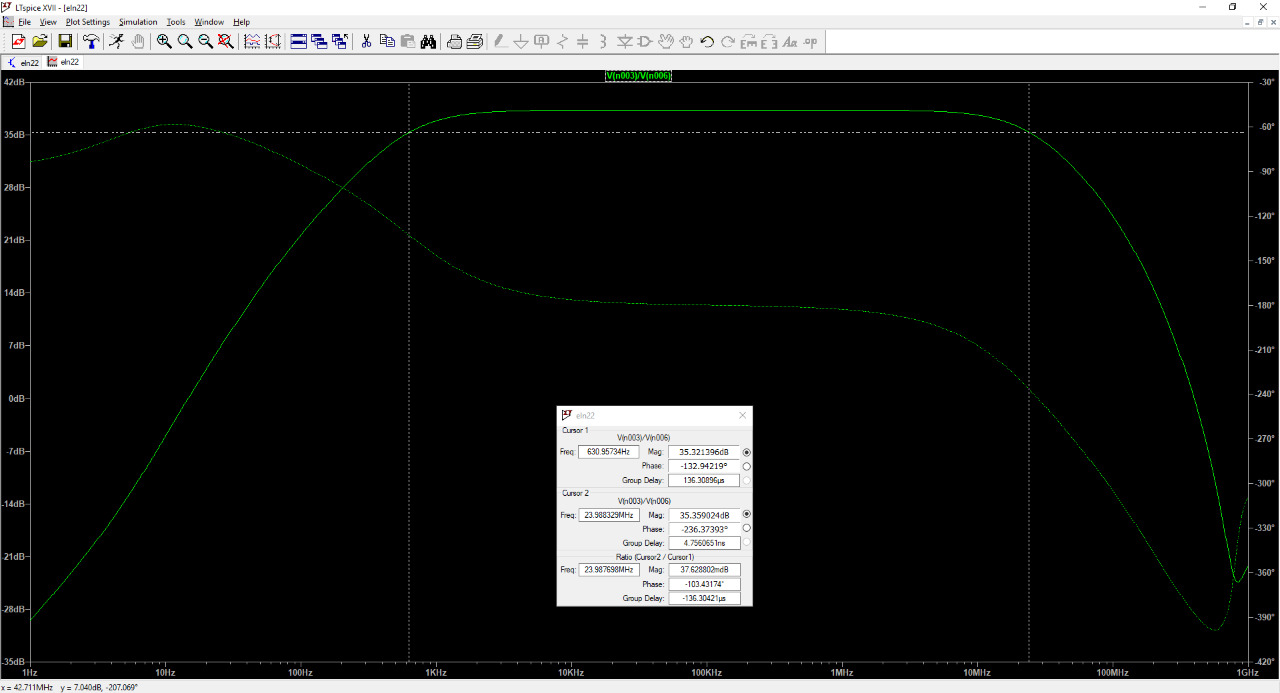
\includegraphics[width=\columnwidth]{Ganho.jpeg}
        		\caption{Ganho A\textsubscript{v} e frequência de corte inferior f\textsubscript{L} e superior f\textsubscript{H} do circuito Cascode.}
        		\label{Ganho1}
        		\end{center}
    	    \end{figure}
    	 
        \tab Percebe-se que a frequência de corte inferior f\textsubscript{L} simulada é de 630 Hz, enquanto a frequência de corte superior f\textsubscript{H} é, aproximadamente, 66,06 MHz. Ainda, é possível notar que o ganho de tensão A\textsubscript{v}, sem considerar o efeito de R\textsubscript{L}, é em torno de 38,5 dB.
        
        \tab Além disso, verificou-se o comportamento de f\textsubscript{L} ao variar as capacitâncias $C_{in}$, $C_1$ e $C_E$ e $C_L$. Conclui-se que a mudança de $C_{in}$, $C_1$ e $C_E$ não alteram de forma significativa o valor de f\textsubscript{L}. No entanto, a alteração de $C_E$ de $10 \: \mu F$ para $100 \: \mu F$ e para $1000 \: \mu F$ causou uma mudança considerável no valor de f\textsubscript{L} para aproximadamente 66 Hz. Observa-se essa mudança nas Figuras \ref{fl ce1} e \ref{fl ce2}.
            
            \begin{figure}[H]
        		\begin{center}
        		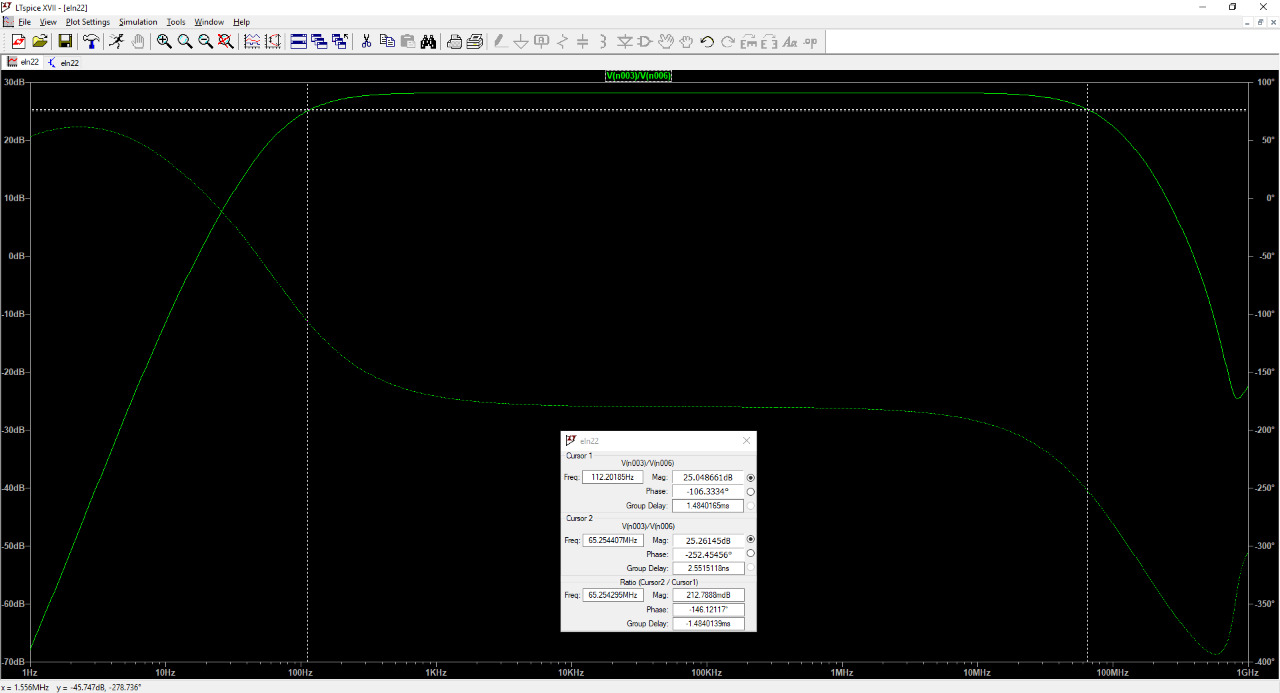
\includegraphics[width=\columnwidth]{100.jpeg}
        		\caption{Frequência de corte inferior f\textsubscript{L} do circuito Cascode para $C_E$ igual à $100 \: \mu F$.}
        		\label{fl ce1}
        		\end{center}
    	    \end{figure}
    	    
    	    \begin{figure}[H]
        		\begin{center}
        		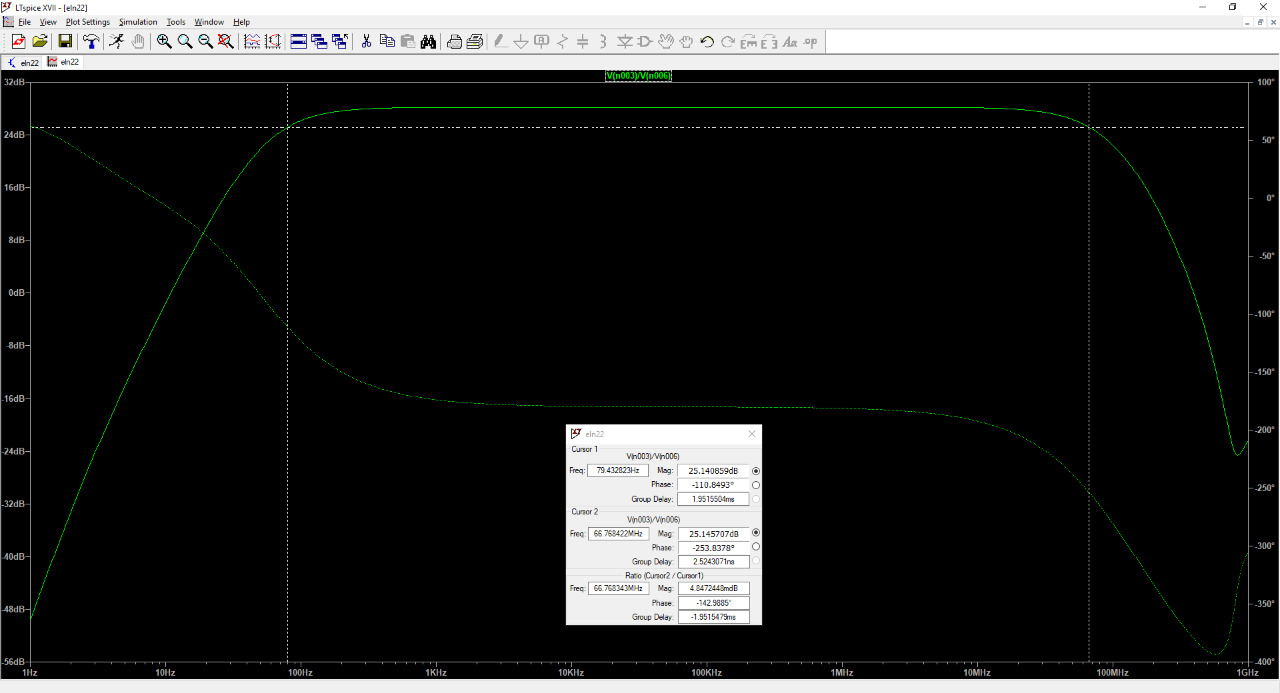
\includegraphics[width=\columnwidth]{1000.jpeg}
        		\caption{Frequência de corte inferior f\textsubscript{L} do circuito Cascode para $C_E$ igual à $1000 \: \mu F$.}
        		\label{fl ce2}
        		\end{center}
    	    \end{figure}
        \tab Como última análise sem a consideração do R\textsubscript{L}, observa-se, agora, o ganho de corrente da configuração Cascode:
        
              \begin{figure}[H]
        		\begin{center}
        		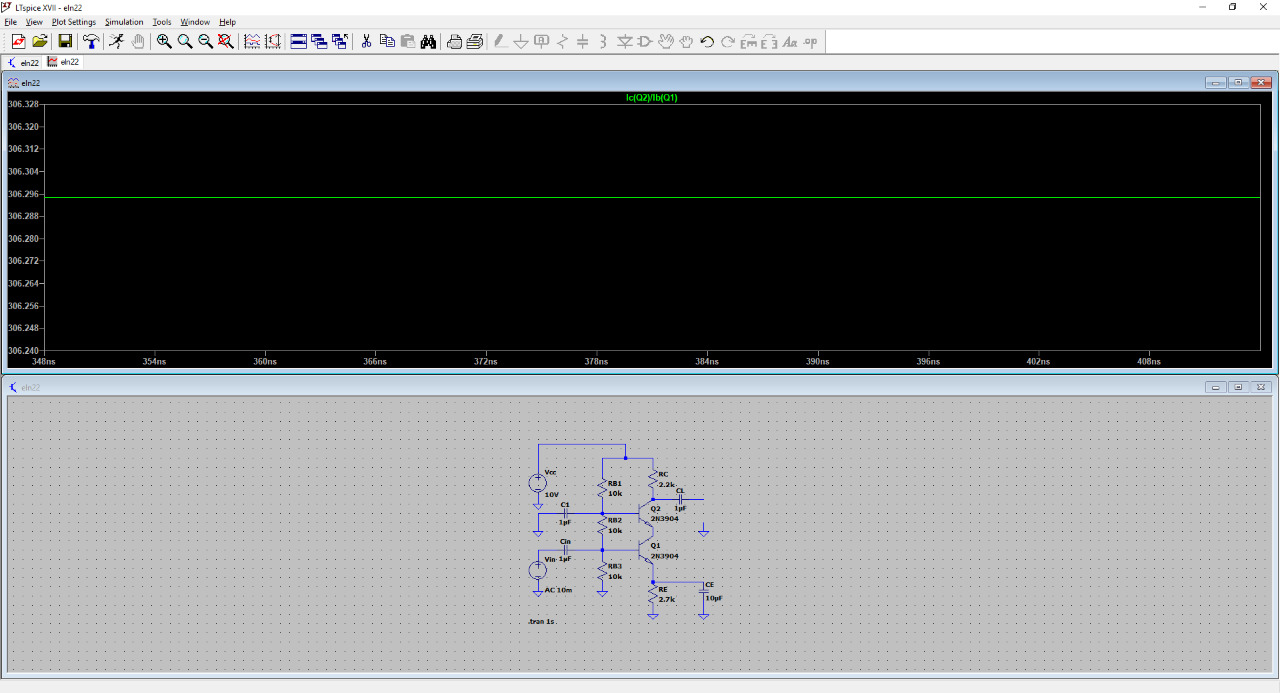
\includegraphics[width=\columnwidth]{beta1.jpeg}
        		\caption{Ganho de corrente da configuração Cascode, sem R\textsubscript{L}}
        		\label{beta1}
        		\end{center}
    	    \end{figure}
        
        \tab Agora, ao considerar o efeito de R\textsubscript{L}, pode-se ver que a variação do ganho de corrente associado a essa configuração não é significante. Observe-se na figura \ref{beta2}

            \begin{figure}[H]
        		\begin{center}
        		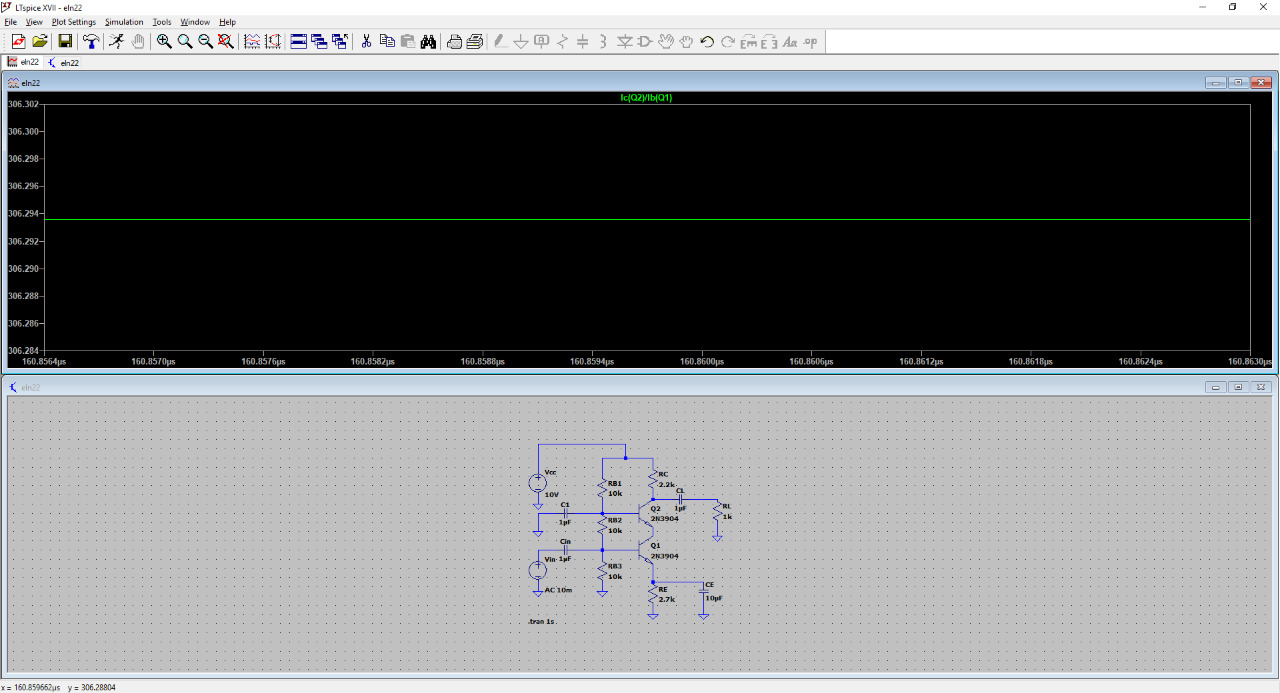
\includegraphics[width=\columnwidth]{beta2.jpeg}
        		\caption{Ganho de corrente da configuração Cascode, com R\textsubscript{L}}
        		\label{beta2}
        		\end{center}
    	    \end{figure}
    	 \tab Por último, observa-se o ganho de tensão, com o efeito de R\textsubscript{L} na figura abaixo:
    	
    	     \begin{figure}[H]
        		\begin{center}
        		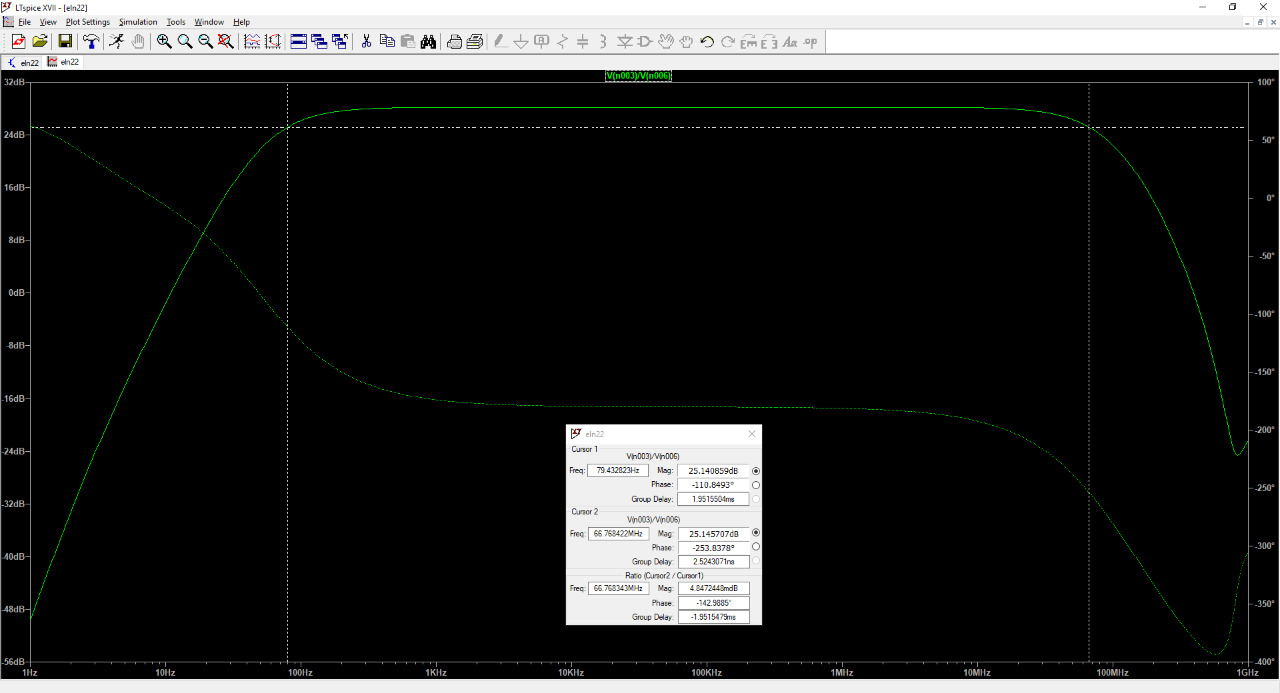
\includegraphics[width=\columnwidth]{Ganho2.jpeg}
        		\caption{Ganho de tensão A\textsubscript{v} da configuração Cascode, com R\textsubscript{L}}
        		\label{Ganho2}
        		\end{center}
    	    \end{figure}
    	  \tab É evidente, a partir da Figuras \ref{Ganho1} e \ref{Ganho2}, que o ganho de tensão, levando em consideração o efeito de R\textsubscript{L}, é de, aproximadamente, 28 dB. Portanto, a variação de ganho de tensão por conta da presença de r\textsubscript{L }é de, aproximadamente, 10,5 dB, ou, 3,35 V/V de variação.
        
        
        
        
        
        
\section{Equipamentos Utilizados}
    \tab Durante a prática, os seguintes instrumentos foram utilizados para a montagem e avaliação do circuito:
     \begin{itemize}
        \item Multímetro digital.
        
        \item Osciloscópio com gerador de sinais.
        
        \item Fonte de alimentação contínua.
        
        \item \textit{Protoboard}.
        
        \item Dois transistores NPN.
        
        \item Resistores de $10 \: k\Omega,\: 2,7 \: k\Omega, e \:2,2 \: k\Omega$.
        
        \item Capacitores de $1 \: \mu F,\: 10 \: \mu F$ e $100 \: \mu F$ e $1000 \: \mu F$.
        
     \end{itemize}
    
        
\section{Procedimento Experimental}

    \tab O circuito sugerido foi montado com os respectivos componentes comprados pela equipe e o osciloscópio foi usado para determinar o ganho de tensão ao qual o sinal foi submetido. Depois, aumentou-se a amplitude do sinal de entrada até verificar-se saturação ou corte, anotando-se a amplitude responsável pela distorção. Alterou-se o valor da frequência até identificar-se as frequências de corte, f\textsubscript{H}, e de saturação, f\textsubscript{L}, do circuito. Por último, a observação anterior foi repetida, trocando-se os valores de C\textsubscript{E} e anotando-se f\textsubscript{L} para cada caso.
    
    \begin{figure}[H]
    	\begin{center}
    	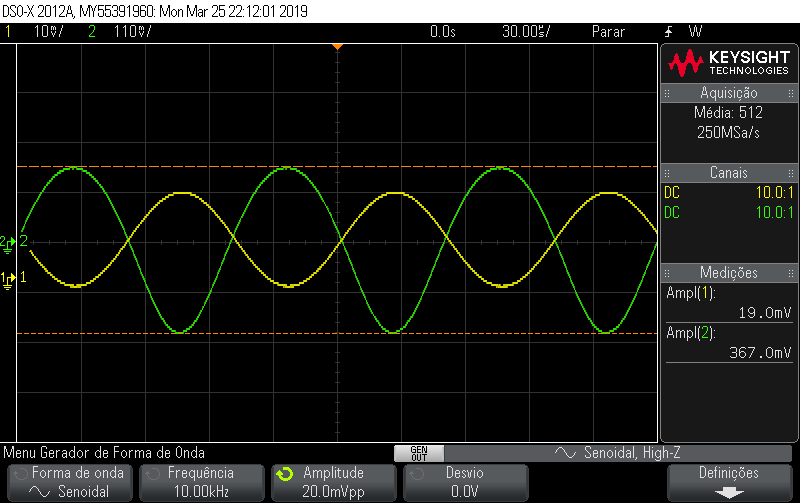
\includegraphics[width=\columnwidth]{Ganho Cascode.png}
    	\caption{Ganho A\textsubscript{V} real da configuração Cascode}
    	\label{Ganho real}
        \end{center}
    \end{figure}
    
    \begin{figure}[H]
    	\begin{center}
    	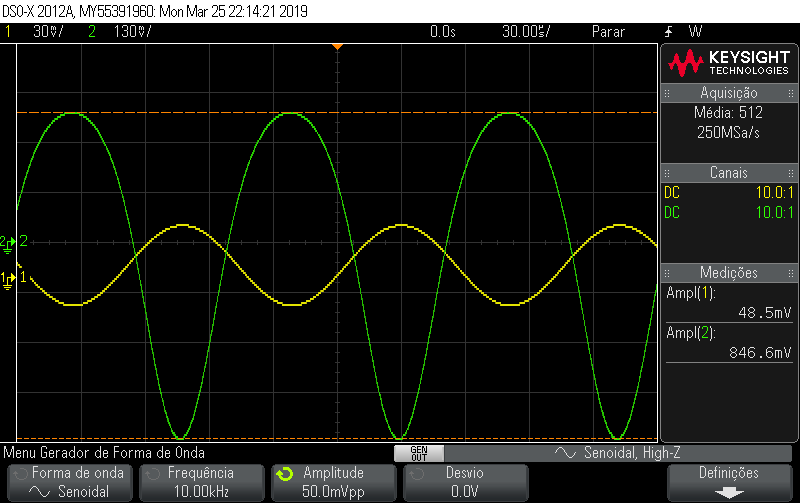
\includegraphics[width=\columnwidth]{GanhoSat.png}
    	\caption{Ganho máximo antes da saturação}
    	\label{Ganho Saturação}
        \end{center}
    \end{figure}
    
    \begin{figure}[H]
      \begin{center}
      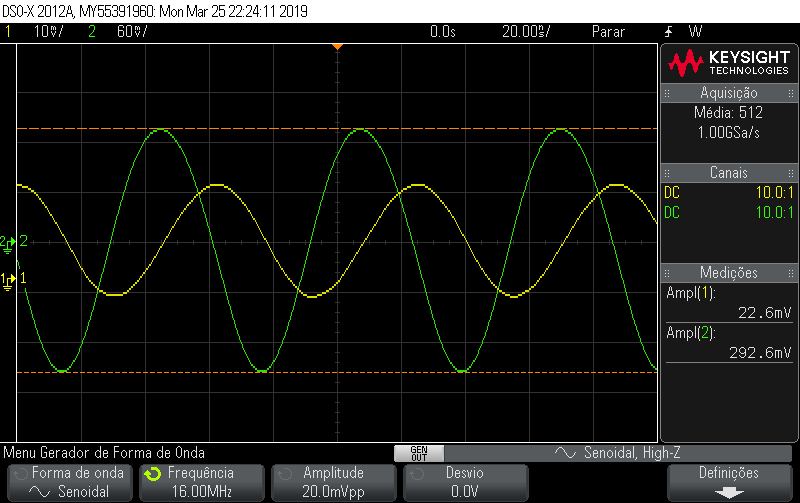
\includegraphics[width=\columnwidth]{FH.png}
      \caption{Frequência f\textsubscript{H} para C\textsubscript{E} como $10 \: \mu F$}
      \label{FH}
      \end{center}
    \end{figure}  
    
    \begin{figure}[H]
        \begin{center}
        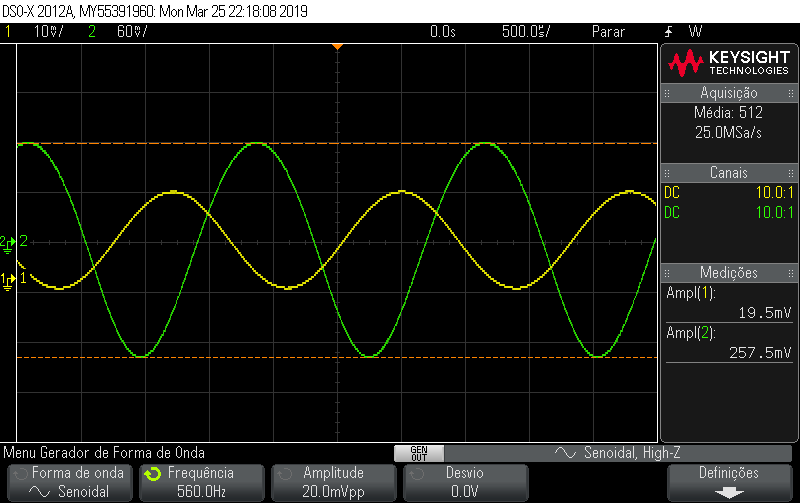
\includegraphics[width=\columnwidth]{FL.png}
        \caption{Frequência f\textsubscript{L} para C\textsubscript{E} como $10 \: \mu F$}
        \label{FL}
        \end{center}
    \end{figure}
    
    \begin{figure}[H]
        \begin{center}
        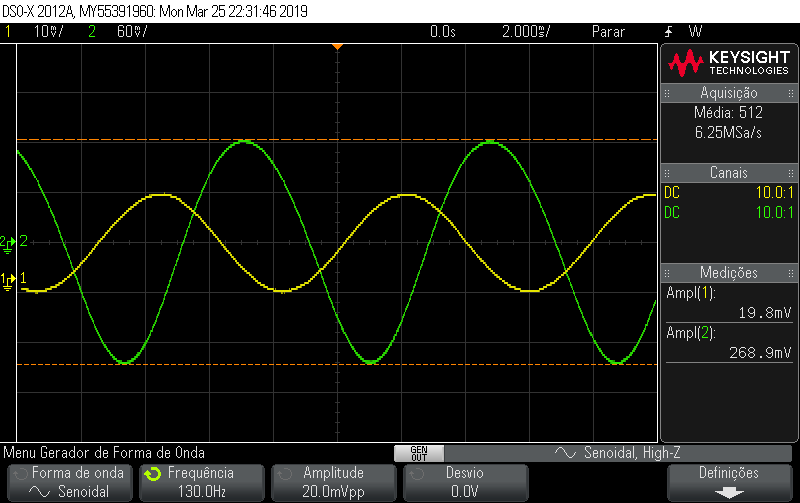
\includegraphics[width=\columnwidth]{100micro.png}
        \caption{Frequência f\textsubscript{L} para C\textsubscript{E} como $100 \: \mu F$}
        \label{fl_100}
        \end{center}
    \end{figure}
    
    \begin{figure}[H]
        \begin{center}
        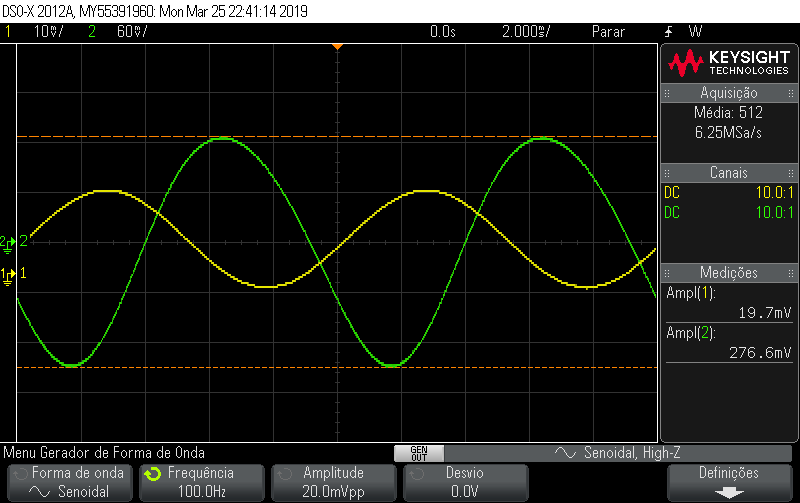
\includegraphics[width=\columnwidth]{1000micro.png}
        \caption{Frequência f\textsubscript{L} para C\textsubscript{E} como $1000 \: \mu F$}
        \label{fl_1000}
        \end{center}
    \end{figure}
    
\section{Análise dos resultados}
    \tab Como realizado anteriormente na etapa de simulação, o circuito montado foi observado, desta vez com o uso de um osciloscópio, e as imagens geradas, anexas à seção anterior, serão discutidas abaixo:
     Na figura \ref{Ganho real}, observa-se a evidente discrepância entre o valor simulado e aquele obtido em prática. Este desvio é de aproximadamente 8,15\%. Um erro desta magnitude é considerado razoável para esta prática, já que os componentes utilizados não são exatamente aqueles usados na construção do projeto de circuito. Ainda, como este circuito não é integrado, está sujeito a diversas interferências externas como, por exemplo, a protoboard ou os erros aleatórios causados pela ação humana do grupo ao implementar o circuito na prática. Julga-se, portanto, que este circuito está suficientemente próximo, no quesito ganho de tensão, àquilo proposto pelo grupo anteriormente.
    
    \tab A imagem \ref{Ganho Saturação} revela que a real amplitude do sinal de entrada para a qual existe saturação no transistor Darlington é 48,5 mV (pico-a-pico). Ainda, observando as imagens \ref{FH} e \ref{FL}, pode-se obter os valores de FH e FL como 16 MHz e 560 Hz, respectivamente.
    
    \tab Observando as imagens \ref{FL}, \ref{fl_100} e \ref{fl_1000}, pode-se tirar as seguintes conclusões: mudando os valores de C\textsubscript{E}, observou-se, como esperado, que a variação da frequência de corte do circuito é dominante e, portanto,é aquela que define a ordem de grandeza da frequência inferior f\textsubscript{L}. Entretanto, quando se aumenta o valor das demais capacitâncias, f\textsubscript{L} tem seu valor atenuado de maneira desprezível. No projeto do circuito, obteve-se o valor de f\textsubscript{L} = 840 Hz. Na prática, obteve-se o valor de 560 Hz. O grupo considerou essa diferença como aceitável, já que os valores das resistências, na prática, mudam e, assim, as impedâncias vistas pelos terminais também são alteradas.
    
    \tab 
\end{document}